\usepackage{pgf}
\usepackage{tikz}
\usepackage{pgfplots}
\usepackage{pgfplotstable}
\usetikzlibrary{arrows,automata,fit, shapes, calc, positioning}


\tikzstyle{inputNode}=[draw=white,circle,minimum size=10pt,inner sep=0pt]
\tikzstyle{stateTransition}=[->, thick]
\def\layersep{2.5cm}

\tikzset{
	every node/.style={
		font=\scriptsize
	},
	dinero/.style={
		shape=rectangle,
		minimum height=1cm,
		text width=2cm,
		text centered,
		rounded corners=1ex,
		draw,
		label={[yshift=-0.7cm]left:poco},
		label={[yshift=-0.7cm]right:mucho},
	},
	tiempo/.style={
		shape=rectangle,
		minimum height=1cm,
		text width=2cm,
		text centered,
		rounded corners=1ex,
		draw,
		label={[yshift=-0.7cm]left:soleado},
		label={[yshift=-0.7cm]right:lluvioso},
	},
	outcome/.style={
		shape=ellipse,
		fill=gray!15,
		draw,
		text width=1.5cm,
		text centered
	},
	decision tree/.style={
		edge from parent path={[-latex] (\tikzparentnode) -| (\tikzchildnode)},
		sibling distance=3cm,
		level distance=1.125cm
	}
}

\tikzset{
	every node/.style={
		font=\scriptsize
	},
	moroso/.style={
		shape=rectangle,
		minimum height=1cm,
		text width=2cm,
		text centered,
		rounded corners=1ex,
		draw,
		label={[yshift=-0.7cm]left:sí},
		label={[yshift=-0.7cm]right:no},
	},
	ingresos/.style={
		shape=rectangle,
		minimum height=1cm,
		text width=2cm,
		text centered,
		rounded corners=1ex,
		draw,
		label={[yshift=-0.25cm]left:$<600$},
		label={[yshift=-0.25cm]right:$600-1200$},
		label={[yshift=-0.1cm, xshift=0.5cm]below:$>1200$},
	},
	outcome/.style={
		shape=ellipse,
		fill=gray!15,
		draw,
		text width=1.5cm,
		text centered
	},
	decision tree/.style={
		edge from parent path={[-latex] (\tikzparentnode) -- (\tikzchildnode)},
		sibling distance=3cm,
		level distance=1.125cm
	}
}



\newcommand{\arboldedecision}{
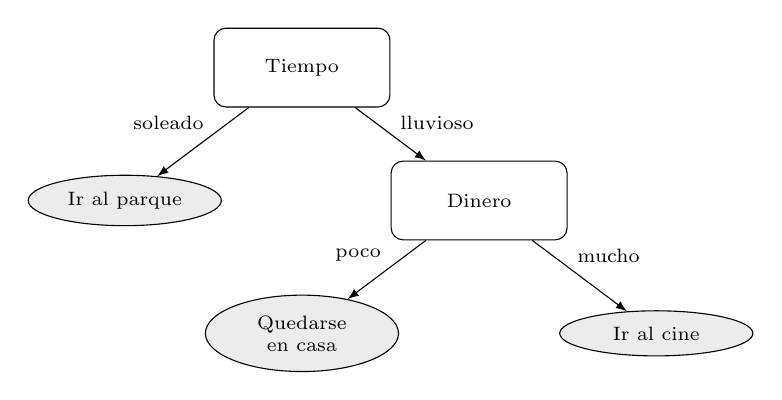
\begin{tikzpicture}[scale = 1.5]
\node [tiempo] {Tiempo }
[decision tree]
child { node [outcome] {Ir al parque} }
child { node [dinero] { Dinero } 
	child { node [outcome] { Quedarse en casa } }
	child { node [outcome] { Ir al cine } }
};
\end{tikzpicture}	
}

\newcommand{\ejemploarboldecision}{
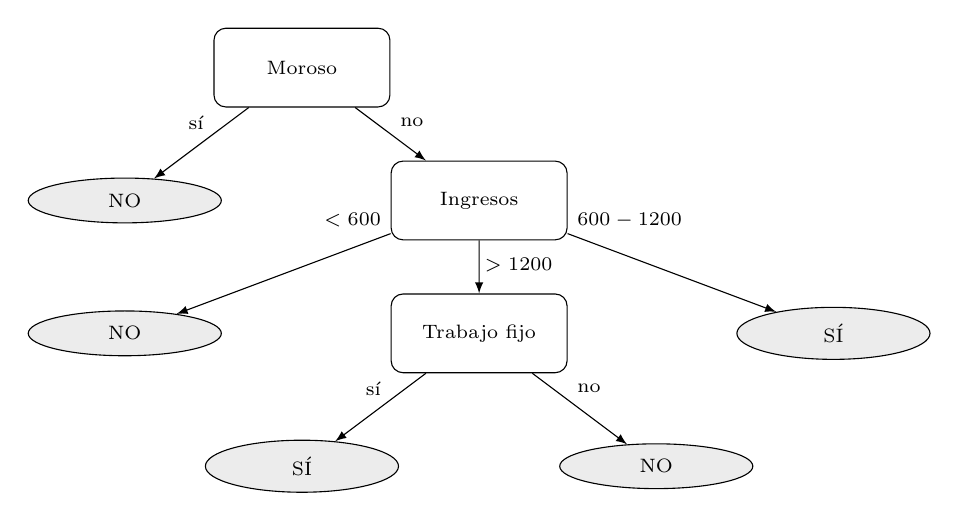
\begin{tikzpicture}[scale = 1.5]

\node [moroso] {Moroso}[decision tree]
child { node [outcome] {NO} }
child { node [ingresos] { Ingresos } 
	child { node [outcome] { NO } }
	child { node [moroso] {Trabajo fijo}
		child { node [outcome] { SÍ } }
		child { node [outcome] { NO } }
	}
	child { node [outcome] { SÍ } }
};

\end{tikzpicture}	
}

\newcommand{\ejemplografo}{
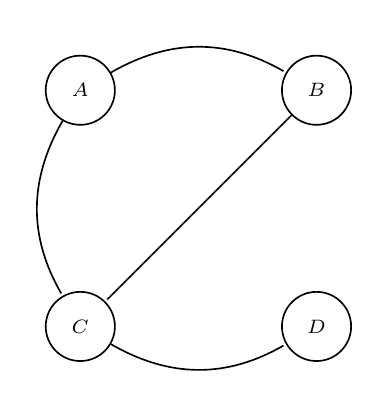
\begin{tikzpicture}[>=stealth',shorten >=1pt,auto,node distance=3cm,semithick]
  \tikzstyle{every state}=[draw=black,text=black]

  \node[state]         (A)                    {$A$};
  \node[state]         (B) [right of=A]       {$B$};
  \node[state]         (C) [below of=A]       {$C$};
  \node[state]         (D) [right of=C]       {$D$};
  
  \path (A) edge  [bend left]   node {}  (B)
            edge  [bend right]  node {}  (C)
        (B) edge                node {}  (C)
        (C) edge  [bend right]  node {}  (D);
\end{tikzpicture}}

\newcommand{\neuronaMcCullochPitts}{
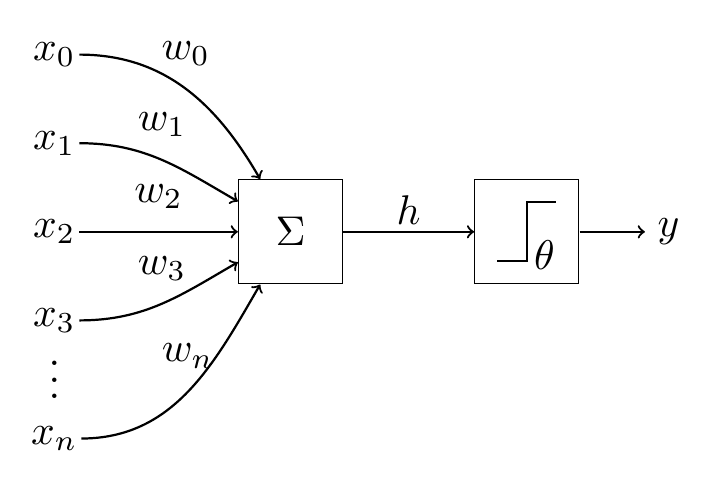
\begin{tikzpicture}[scale=1.5, every node/.style={scale=1.5}]
\node[draw,minimum size=25pt,inner sep=0pt] (x) at (0,0) {$\Sigma$};
\node[draw,minimum size=25pt,inner sep=0pt] (s) at (2,0) {};

\node[inputNode] (x0) at (-2, 1.5) {$x_0$};
\node[inputNode] (x1) at (-2, 0.75) {$x_1$};
\node[inputNode] (x2) at (-2, 0) {$x_2$};
\node[inputNode] (x3) at (-2, -0.75) {$x_3$};
\node[inputNode] (xn) at (-2, -1.75) {$x_n$};

\draw[stateTransition] (x0) to[out=0,in=120] node [above=0.1]  {$w_0$} (x);
\draw[stateTransition] (x1) to[out=0,in=150] node [above=0.1] {$w_1$} (x);
\draw[stateTransition] (x2) to[out=0,in=180] node [above=0.1] {$w_2$} (x);
\draw[stateTransition] (x3) to[out=0,in=210] node [above=0.1] {$w_3$} (x);
\draw[stateTransition] (xn) to[out=0,in=240] node [above=0.1] {$w_n$} (x);

\draw[stateTransition] (x) -- (s) node [midway,above=-0.1cm] {$h$};
\draw[stateTransition] (s) -- (3,0) node [midway,above=-0.1cm] {};
\node[draw=none] at (3.2,0) {$y$};

\node (dots) at (-2, -1.15) {$\vdots$};

\draw[thick] (1.75,-0.25) -- (2,-0.25) -- (2, 0.25) -- (2.25,0.25);
\node[draw=none] at (2.15,-0.2) {$\theta$};
\end{tikzpicture}
}

\newcommand{\perceptron}{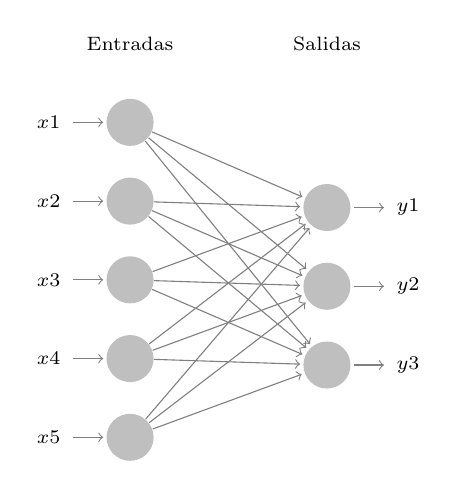
\begin{tikzpicture}
	[shorten >=1pt,->,draw=black!50, node distance=\layersep]
	\tikzstyle{every pin edge}=[<-,shorten <=1pt]
	\tikzstyle{neuron}=[circle,fill=gray!25,minimum size=17pt,inner sep=0pt]
	\tikzstyle{input neuron}=[neuron, fill=gray!50];
	\tikzstyle{output neuron}=[neuron, fill=gray!50];
	\tikzstyle{hidden neuron}=[neuron, fill=gray!50];
	\tikzstyle{annot} = [text width=4em, text centered]
	
	\foreach \name / \y in {1,...,5}
	\node[input neuron, pin=left: $x$\y] (I-\name) at (0,-\y) {};
	
	\foreach \name / \y in {1,...,3}
	\path[yshift=0.5cm]
	node[hidden neuron,pin={[pin edge={->}]right:$y$\y}] (O-\name) at (\layersep,-45-\y cm) {};
	
	\foreach \source in {1,...,5}
	\foreach \dest in {1,...,3}
	\path (I-\source) edge (O-\dest);
	
	\node[annot,above of=I-1, node distance=1cm] (hl) {Entradas};
	\node[annot,right of=hl] {Salidas};
\end{tikzpicture}}

\newcommand{\linealmenteseparable}{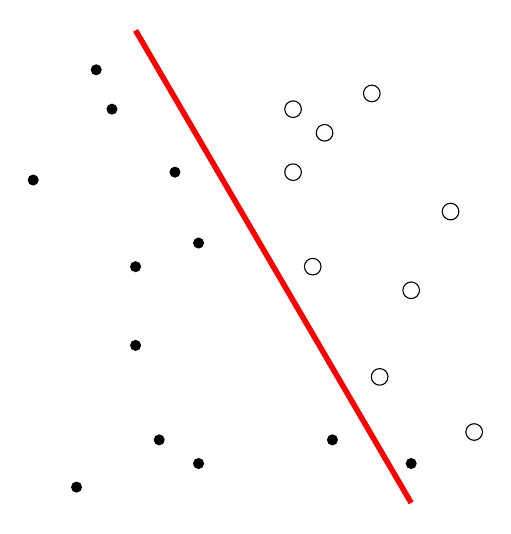
\begin{tikzpicture}
	
	\draw[color=red,line width=2pt] (8.5,6) -- (12,0);
	
	\def\pos{{%
			{9.3,3.3},
			{11,.8},
			{8.5,2},
			{7.2,4.1},
			{8.8,.8},
			{8,5.5},
			{8.2,5},
			{7.75,.2},
			{9,4.2},
			{12, 0.5},
			{8.5,3},
			{9.3,.5},
		}}
		
		\foreach \i in {0,...,11} {
			\pgfmathparse{\pos[\i][0]}\let \x \pgfmathresult;
			\pgfmathparse{\pos[\i][1]}\let \y \pgfmathresult;
			\fill[black] (\x,\y) circle (2pt);
		}
		
		\def\neg{{%
				{10.75,3},
				{10.5,5},
				{11.6,1.6},
				{11.5,5.2},
				{12.5,3.7},
				{10.9,4.7},
				{12,2.7},
				{10.5,4.2},
				{12.8,.9},
			}}
			
			\foreach \i in {0,...,8} {
				\pgfmathparse{\neg[\i][0]}\let \x \pgfmathresult;
				\pgfmathparse{\neg[\i][1]}\let \y \pgfmathresult;
				\draw[black] (\x,\y) circle (3pt);
			}
			
			\end{tikzpicture}}
		
\newcommand{\nolinealmenteseparable}{	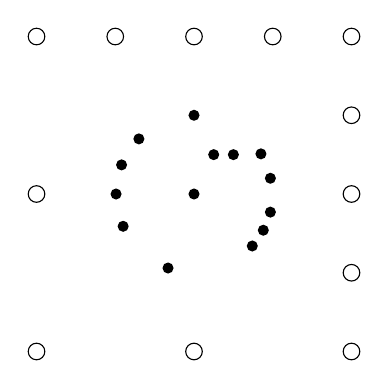
\begin{tikzpicture}
	
	\def\positive{{%
			{0.97,-0.23},
			{-0.33,-0.94},
			{-0.9,-0.41},
			{0.74,-0.66},
			{0.97,0.20},
			{0.88,-0.46},
			{-0.70,0.70},
			{-0.92,0.37},
			{0.85,0.51},
			{-0.99, 0},
			{0,0},
			{0.5,0.5},
			{0,1},
			{0.25, 0.5}
		}}
		
		\foreach \i in {0,...,13} {
			\pgfmathparse{\positive[\i][0]}\let \x \pgfmathresult;
			\pgfmathparse{\positive[\i][1]}\let \y \pgfmathresult;
			\fill[black] (\x,\y) circle (2pt);
		}
		
		\def\negative{{%
				{2,1},
				{1,2},
				{0,2},
				{-1,2},
				{2,-1},
				{2,0},
				{-2,0},
				{-2,-2},
				{0,-2},
				{-2,2},
				{2,2},
				{2,-2}
			}}
			
			\foreach \i in {0,...,11} {
				\pgfmathparse{\negative[\i][0]}\let \x \pgfmathresult;
				\pgfmathparse{\negative[\i][1]}\let \y \pgfmathresult;
				\draw[black] (\x,\y) circle (3pt);
			}
			
			\end{tikzpicture}}

\newcommand{\xor}{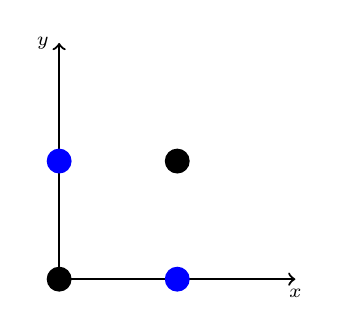
\begin{tikzpicture}[scale=1.5]
	
	\draw [<->,thick] (0,2) node (yaxis) [left] {$y$}
	|- (2,0) node (xaxis) [below] {$x$};
	
	\fill[black] (0,0) circle (3pt);
	\fill[blue] (1,0) circle (3pt);
	\fill[blue] (0,1) circle (3pt);
	\fill[black] (1,1) circle (3pt);
	\end{tikzpicture}}

\newcommand{\perceptronmulticapa}{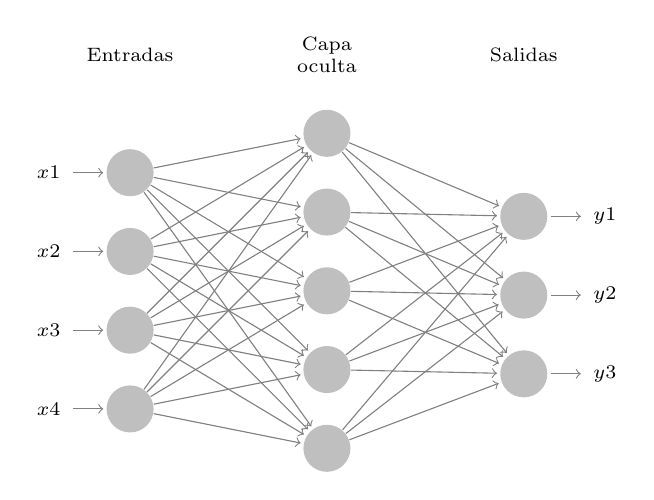
\begin{tikzpicture}
	[shorten >=1pt,->,draw=black!50, node distance=\layersep]
	\tikzstyle{every pin edge}=[<-,shorten <=1pt]
	\tikzstyle{neuron}=[circle,fill=gray!25,minimum size=17pt,inner sep=0pt]
	\tikzstyle{input neuron}=[neuron, fill=gray!50];
	\tikzstyle{output neuron}=[neuron, fill=gray!50];
	\tikzstyle{hidden neuron}=[neuron, fill=gray!50];
	\tikzstyle{annot} = [text width=4em, text centered]
	
	\foreach \name / \y in {1,...,4}
	\node[input neuron, pin=left: $x$\y] (I-\name) at (0,-\y) {};
	
	\foreach \name / \y in {1,...,5}
	\path[yshift=0.5cm]
	node[hidden neuron] (H-\name) at (\layersep,-\y cm) {};
	
	\foreach \name / \y in {1,...,3}
	\path[yshift=0.5cm]
	node[hidden neuron,pin={[pin edge={->}]right:$y$\y}] (O-\name) at (2*\layersep,-30-\y cm) {};
	
	\foreach \source in {1,...,4}
	\foreach \dest in {1,...,5}
	\path (I-\source) edge (H-\dest);
	
	\foreach \source in {1,...,5}
	\foreach \dest in {1,...,3}
	\path (H-\source) edge (O-\dest);
	
	\node[annot,above of=H-1, node distance=1cm] (hl) {Capa oculta};
	\node[annot,left of=hl] {Entradas};
	\node[annot,right of=hl] {Salidas};
\end{tikzpicture}}

\newcommand{\aprendizajerefuerzo}{
	\tikzset{
		every node/.style={
			font=\scriptsize
		},
		node/.style={
			shape=rectangle,
			minimum height=1cm,
			text width=2cm,
			text centered,
			rounded corners=1ex,
			draw,
		},
		myarrow/.style={->},
		myarrow2/.style={<-},        
	}
	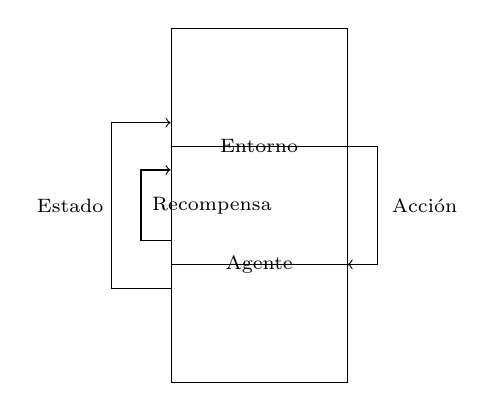
\begin{tikzpicture}[scale = 1.5]
	\node [node] (agt) at (0,1) {Entorno};
	\node [node] (ent) at (0,0) {Agente};
	\draw [myarrow2] (ent.east) -- ++(.25,0) -- ++(0,1) -|  (agt.east);		
	\draw [myarrow] (-0.75, 0.2) -- (-1,0.2) -- (-1,0.8) -- (-0.75,0.8);
	\draw [myarrow] (-0.75,-0.2) -- (-1.25,-0.2) -- (-1.25,1.2) -- (-0.75,1.2);
	
	\node[draw=none] at (1.4,0.5) {Acción};
	\node[draw=none] at (-0.4,0.5) {Recompensa};
	\node[draw=none] at (-1.6,0.5) {Estado};

\end{tikzpicture}}


\tikzset{main node/.style={circle,draw,minimum size=0.5cm,inner sep=0pt},
}

\tikzstyle{every pin edge}=[<-,shorten <=1pt]
	
	\pgfmathsetseed{1138} % set the random seed
	\pgfplotstableset{ % Define the equations for x and y
		create on use/x/.style={create col/expr={42+2*\pgfplotstablerow}},
		create on use/y/.style={create col/expr={(0.6*\thisrow{x}+130)+5*rand}}
	}
	
	\pgfplotstablenew[columns={x,y}]{10}{\loadedtable}
	
	
	\pgfplotstableset{ % Define the equations for x and y
		create on use/x/.style={create col/expr={20+2*\pgfplotstablerow}},
		create on use/y/.style={create col/expr={(0.3*\thisrow{x}+100)+10*rand}}
	}
	
	\pgfplotstablenew[columns={x,y}]{10}{\loadedtableB}
	
	\tikzset{
		every node/.style={
			font=\scriptsize
		},
		node/.style={
			shape=rectangle,
			minimum height=3cm,
			text width=2cm,
			text centered,
			draw,
		},
		myarrow/.style={->},
		myarrow2/.style={<-},        
	}
	
	
	\newcommand{\papel}{
		
\begin{tikzpicture}[scale = 1.5]
		\node [node] at (0,0) {};
		
		\foreach \x in {0,1,2,3,4,5,6,7,8,9}{
			\draw (-0.5,-0.1*\x+0.5) -- coordinate(a\x) (0.5,-0.1*\x +0.5);	}
		
		\end{tikzpicture}}
	\newcommand{\reg}{
		\begin{tikzpicture}[scale = 0.25]
		\begin{axis}[
		axis lines=left,
		xtick=\empty, 
		ytick=\empty
		]
		\addplot [only marks, fill=blue, draw=blue, thick] table {\loadedtable};
		\addplot [no markers, thick, blue] table [y={create col/linear regression={y=y}}] {\loadedtable} node [anchor=west] {};
		\end{axis}
		\end{tikzpicture}}
	
	\newcommand{\regg}{
		\begin{tikzpicture}[scale = 0.25]
		\begin{axis}[
		axis lines=left,
		xtick=\empty, 
		ytick=\empty
		]
		\addplot [only marks, fill=green, draw=green, thick] table {\loadedtableB};
		\addplot [no markers, thick, green] table [y={create col/linear regression={y=y}}] {\loadedtableB} node [anchor=west] {};
		\end{axis}
		\end{tikzpicture}}
	
	\newcommand{\regresionplot}{
		\begin{tikzpicture}
		\node[]() at (0,0) {\reg} ;
		\node[]() at (0,1.5) {\regg};
		\end{tikzpicture}}
	
	\newcommand{\grafo}{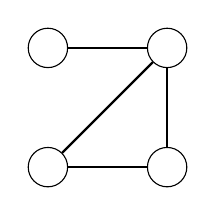
\begin{tikzpicture}
		
		\node[main node] (1) {};
		\node[main node] (2) [right = 1cm  of 1]  {};
		\node[main node] (3) [below = 1cm  of 1] {};
		\node[main node] (4) [right = 1cm  of 3] {};
		
		\path[draw,thick]
		(1) edge node {} (2)
		(2) edge node {} (4)
		(3) edge node {} (4)
		(2) edge node {} (3);
		
		\end{tikzpicture}}
	
	\newcommand{\redesparencliticas}{\begin{tikzpicture}
	\node[](a) at (0,0) {\papel};
	\node[](b) at (4,0) {\regresionplot};
	\node[](c) at (7.5,0) {\grafo};
	\node[pin={[pin edge={->}]right:Clasificación}](d) at (12,0) {\papel};
	
	\draw [->] (a) -> node[midway,fill=white] {Regresión} (b);
	\draw [->] (b) -> (c);
	\draw [->] (c) -> node[midway,fill=white] {Medidas} (d);
	
	\end{tikzpicture}}

\newcommand{\clasificador}{
	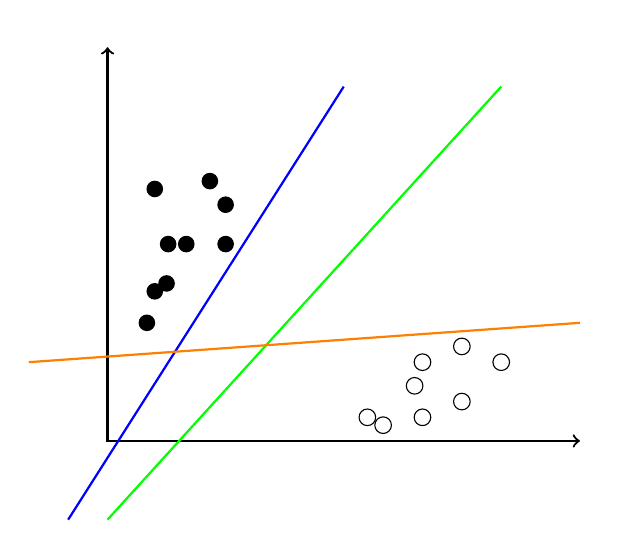
\begin{tikzpicture}
	
	
	\draw [<->,thick] (0,5) node (yaxis) [above] {}
	|- (6,0) node (xaxis) [right] {};
	
	
	\draw[draw=blue, thick] (-0.5,-1) -- (3,4.5); % y=x-1	
	\draw[draw=green, thick] (0,-1) -- (5,4.5); % y=x-1
	\draw[draw=orange, thick] (-1,1) -- (6,1.5); % y=x-1
	
	\fill[black] (0.5,1.5) circle (3pt);
	\fill[black] (1.5,2.5)   circle (3pt);
	\fill[black] (1,2.5)     circle (3pt);
	\fill[black] (0.75,2)    circle (3pt);
	\fill[black] (0.6,1.9)   circle (3pt);
	\fill[black] (0.77, 2.5) circle (3pt);
	\fill[black] (1.5,3)     circle (3pt);
	\fill[black] (1.3,3.3)   circle (3pt);
	\fill[black] (0.6,3.2)   circle (3pt);
	% draw positive dots
	\draw[black] (4,1)     circle (3pt); 
	\draw[black] (3.3,.3)  circle (3pt); 
	\draw[black]     (4.5,1.2) circle (3pt); 
	\draw[black]     (4.5,.5)  circle (3pt); 
	\draw[black]     (3.9,.7)  circle (3pt); 
	\draw[black]     (5,1)     circle (3pt); 
	\draw[black]     (3.5,.2)  circle (3pt); 
	\draw[black]     (4,.3)    circle (3pt); 
	\end{tikzpicture}
}

\newcommand{\margen}{
		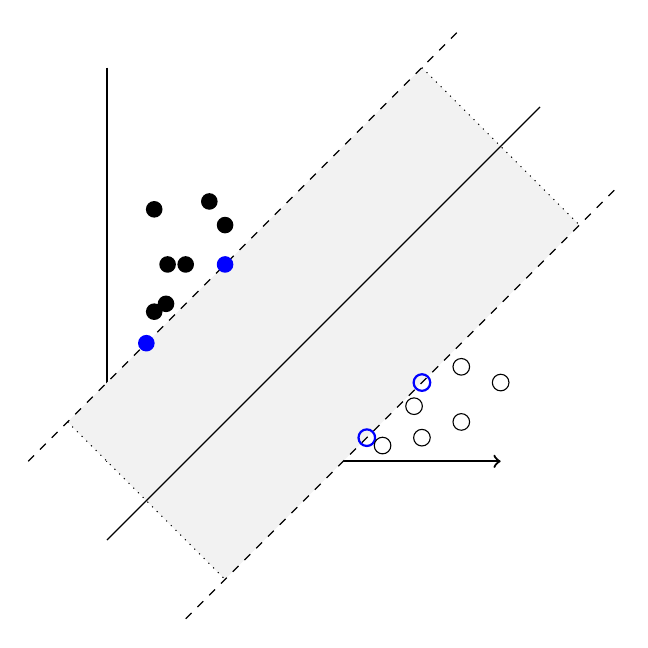
\begin{tikzpicture}
		
		\draw [->,thick] (0,5) node (yaxis) [above] {}
		|- (5,0) node (xaxis) [right] {};
		% draw line
		\draw[fill=gray!10, draw=none] (1.5,-1.5) -- (-0.5,0.5) -- (4,5) -- (6,3) --  cycle;
		\draw (0,-1) -- (5.5,4.5); % y=x-1
		\draw[dashed] (-1,0) -- (4.5,5.5); % y=x+1
		\draw[dashed] (1,-2) -- (6.5,3.5); % y=x-3
		
		\draw[dotted] (4,5) -- (6,3);
		\draw[dotted] (-0.5,0.5) -- (1.5,-1.5);
		
		\fill[blue] (0.5,1.5) circle (3pt);
		\fill[blue]   (1.5,2.5)   circle (3pt);
		\fill[black] (1,2.5)     circle (3pt);
		\fill[black] (0.75,2)    circle (3pt);
		\fill[black] (0.6,1.9)   circle (3pt);
		\fill[black] (0.77, 2.5) circle (3pt);
		\fill[black] (1.5,3)     circle (3pt);
		\fill[black] (1.3,3.3)   circle (3pt);
		\fill[black] (0.6,3.2)   circle (3pt);
		% draw positive dots
		\draw[blue,thick] (4,1)     circle (3pt); 
		\draw[blue,thick] (3.3,.3)  circle (3pt); 
		\draw[black]     (4.5,1.2) circle (3pt); 
		\draw[black]     (4.5,.5)  circle (3pt); 
		\draw[black]     (3.9,.7)  circle (3pt); 
		\draw[black]     (5,1)     circle (3pt); 
		\draw[black]     (3.5,.2)  circle (3pt); 
		\draw[black]     (4,.3)    circle (3pt); 
		\end{tikzpicture}
}

\newcommand{\kernel}{
	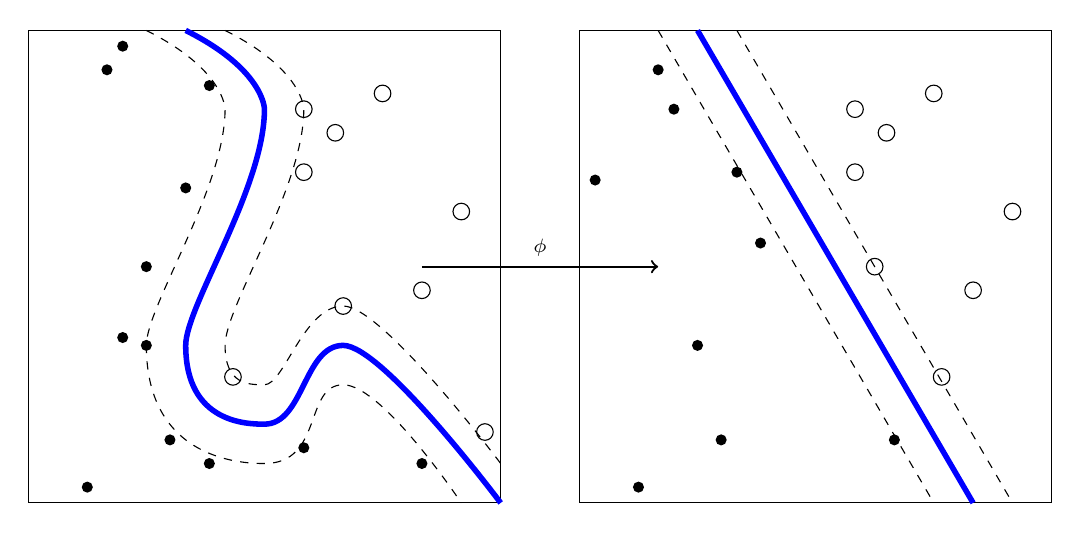
\begin{tikzpicture}
	
	\draw (0,0) rectangle (6,6);
	
	\draw[color=blue,line width=2pt]
	(2,6) .. controls (3,5.5) and (3,5) .. 
	(3,5) .. controls (3,4) and (2,2.5) .. 
	(2,2) .. controls (2,1) and (2.8,1) .. 
	(3,1) .. controls (3.5,1) and (3.5,2) .. 
	(4,2) .. controls (4.5,2) and (6,0) .. 
	(6,0);
	
	\draw[dashed] 
	(1.5,6) .. controls (2.5,5.5) and (2.5,5) .. 
	(2.5,5) .. controls (2.5,4) and (1.5,2.5) .. 
	(1.5,2) .. controls (1.5,.5) and (2.8,.5) .. 
	(3,.5) .. controls (3.75,.5) and (3.5,1.5) .. 
	(4,1.5) .. controls (4.5,1.5) and (5.5,0) .. 
	(5.5,0);
	
	\draw[dashed] 
	(2.5,6) .. controls (3.5,5.5) and (3.5,5) .. 
	(3.5,5) .. controls (3.5,4) and (2.5,2.5) .. 
	(2.5,2) .. controls (2.5,1.5) and (2.8,1.5) .. 
	(3,1.5) .. controls (3.25,1.5) and (3.5,2.5) .. 
	(4,2.5) .. controls (4.5,2.5) and (6,0.5) .. 
	(6,0.5);
	
	\draw (7,0) rectangle (13,6);
	
	\draw[color=blue,line width=2pt] (8.5,6) -- (12,0);
	
	\draw[dashed]  (8,6) -- (11.5,0);
	\draw[dashed]  (9,6) -- (12.5,0);
	
	\draw[thick,->] (5,3) -- (8,3) node [above,pos=.5] {$\phi$};
	
	\def\positive{{%
			{2.3,5.3},
			{3.5,.7},
			{1.5,2},
			{1.2,2.1},
			{1.8,.8},
			{1,5.5},
			{1.2,5.8},
			{.75,.2},
			{2,4},
			{5, 0.5},
			{1.5,3},
			{2.3,.5},
			%
			{9.3,3.3},
			{11,.8},
			{8.5,2},
			{7.2,4.1},
			{8.8,.8},
			{8,5.5},
			{8.2,5},
			{7.75,.2},
			{9,4.2},
			{12, 0.5},
			{8.5,3},
			{9.3,.5},
		}}
		
		\foreach \i in {0,...,20} {
			\pgfmathparse{\positive[\i][0]}\let \x \pgfmathresult;
			\pgfmathparse{\positive[\i][1]}\let \y \pgfmathresult;
			\fill[black] (\x,\y) circle (2pt);
		}
		
		\def\negative{{%
				{4,2.5},
				{3.5,5},
				{2.6,1.6},
				{4.5,5.2},
				{5.5,3.7},
				{3.9,4.7},
				{5,2.7},
				{3.5,4.2},
				{5.8,.9},
				%
				{10.75,3},
				{10.5,5},
				{11.6,1.6},
				{11.5,5.2},
				{12.5,3.7},
				{10.9,4.7},
				{12,2.7},
				{10.5,4.2},
				{12.8,.9},
			}}
			
			\foreach \i in {0,...,16} {
				\pgfmathparse{\negative[\i][0]}\let \x \pgfmathresult;
				\pgfmathparse{\negative[\i][1]}\let \y \pgfmathresult;
				\draw[black] (\x,\y) circle (3pt);
			}
			
			\end{tikzpicture}
}

\newcommand{\ejemplografocompleto}{
	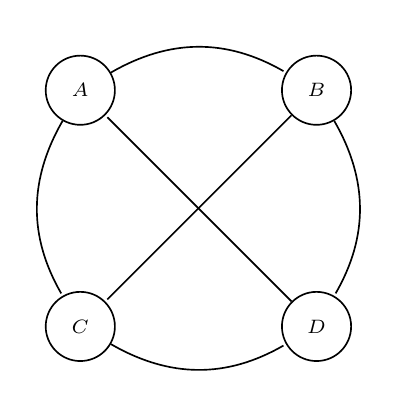
\begin{tikzpicture}[>=stealth',shorten >=1pt,auto,node distance=3cm,semithick]
	\tikzstyle{every state}=[draw=black,text=black]
	
	\node[state]         (A)                    {$A$};
	\node[state]         (B) [right of=A]       {$B$};
	\node[state]         (C) [below of=A]       {$C$};
	\node[state]         (D) [right of=C]       {$D$};
	
	\path (A) edge  [bend left]   node {}  (B)
	edge  [bend right]  node {}  (C)
	(B) edge  [bend left]   node {}  (D)
	(B) edge                node {}  (C)
	(D) edge                node {}  (A)
	(C) edge  [bend right]  node {}  (D);
	\end{tikzpicture}}

\newcommand{\ejemplounionintersecciongrafo}{
	\begin{tikzpicture}[>=stealth',shorten >=1pt,auto,node distance=2cm,semithick]
	\tikzstyle{every state}=[draw=black,text=black]
	
	% Grafo G
	\node[state]         (A)                          {$A$};
	\node[state]         (B) [below right of=A]       {$B$};
	\node[state]         (C) [below      of= B]       {$C$};
	\node[state]         (D) [right of=B]             {$D$};
	\node[state]         (E) [right of=C]             {$E$};
	
	\path (A) edge                node {}  (B)
	(B) edge                node {}  (C)
	(B) edge                node {}  (D)      
	(C) edge                node {}  (E)
	(D) edge                node {}  (E);
	
	% Grafo G'
	\node[state]         (H) [right of= E]       {$C$};
	\node[state]         (I) [right of= D]       {$D$};
	\node[state]         (G) [right of= H]       {$E$};
	\node[state]         (F) [above right of= G] {$F$};
	
	\path (H) edge                node {}  (I)
	(I) edge                node {}  (F)
	(G) edge                node {}  (F)
	(H) edge                node {}  (G);
	
	% Etiquetas con el nombre de los grafos
	\node[align=center, below right of=C] (Z) {$G$};
	\node[align=center, below right of=H] (Y) {$G'$};
	
	% Grafo G \cup G'
	\node[state]         (J) [below left of=Z]        {$A$};
	\node[state]         (K) [below right of=J]       {$B$};
	\node[state]         (L) [below of= K]            {$C$};
	\node[state]         (M) [right of=K]             {$D$};
	\node[state]         (N) [right of=L]             {$E$};
	\node[state]         (R) [above right of=N]       {$F$};
	
	\path (J) edge                node {}  (K)
	(K) edge                node {}  (L)
	(K) edge                node {}  (M)      
	(L) edge                node {}  (N)
	(L) edge                node {}  (M)
	(N) edge                node {}  (R)
	(R) edge                node {}  (M)
	(M) edge                node {}  (N);
	
	\node[align=center, below right of=L] {$G \cup G'$};
	
	% Grafo G \cup G'
	\node[state]         (O) [right of=R]        {$C$};
	\node[state]         (P) [right of=O]              {$E$};
	
	
	\path (O) edge                node {}  (P);
	
	
	\node[align=center, below right of=O] {$G \cap G'$};
	
	\end{tikzpicture}}

\newcommand{\ejemplosubgrafo}{
	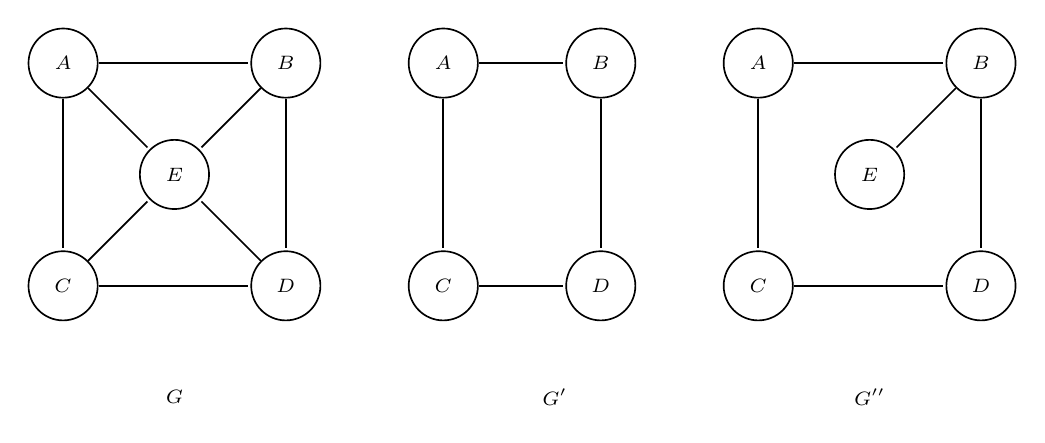
\begin{tikzpicture}[>=stealth',shorten >=1pt,auto,node distance=2cm,semithick]
	\tikzstyle{every state}=[draw=black,text=black]
	
	% Grafo G
	\node[state]         (E)                          {$E$};
	\node[state]         (B) [above right of=E]       {$B$};
	\node[state]         (A) [above left of= E]       {$A$};
	\node[state]         (C) [below left of= E]       {$C$};
	\node[state]         (D) [below right of=E]       {$D$};
	
	\path (A) edge                node {}  (B)
	(A) edge                node {}  (E)
	(A) edge                node {}  (C)
	(B) edge                node {}  (D)
	(B) edge                node {}  (E)        
	(C) edge                node {}  (E)
	(C) edge                node {}  (D)
	(D) edge                node {}  (E);
	
	
	% Subgrafo G'
	\node[state]         (F) [right of= B]       {$A$};
	\node[state]         (G) [right of= F]       {$B$};
	\node[state]         (H) [right of= D]       {$C$};
	\node[state]         (I) [right of= H]       {$D$};
	
	\path (F) edge                node {}  (G)
	(F) edge                node {}  (H)
	(G) edge                node {}  (I)
	(H) edge                node {}  (I);
	
	% Subgrafo G'
	
	\node[state]         (J) [right of= G]             {$A$};
	\node[state]         (K) [right of= I]             {$C$};
	\node[state]         (N) [above right of= K]       {$E$};
	\node[state]         (M) [below right of= N]       {$D$};
	\node[state]         (L) [above right of= N]       {$B$};
	
	\path (J) edge                node {}  (K)
	(J) edge                node {}  (L)
	(L) edge                node {}  (N)
	(L) edge                node {}  (M)
	(K) edge                node {}  (M);
	
	% Etiquetas con el nombre de los grafos
	\node[align=center, below right of=C] {$G$};
	\node[align=center, below right of=H] {$G'$};
	\node[align=center, below right of=K] {$G''$};
	\end{tikzpicture}}

\newcommand{\ejemplografodirigido}{
	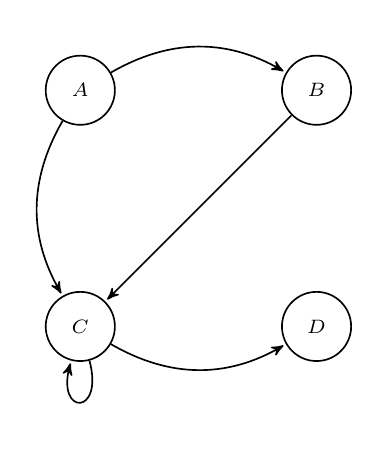
\begin{tikzpicture}[->,>=stealth',shorten >=1pt,auto,node distance=3cm,semithick]
	\tikzstyle{every state}=[draw=black,text=black]
	
	\node[state]         (A)                    {$A$};
	\node[state]         (B) [right of=A]       {$B$};
	\node[state]         (C) [below of=A]       {$C$};
	\node[state]         (D) [right of=C]       {$D$};
	
	\path (A) edge  [bend left]   node {}  (B)
	edge  [bend right]  node {}  (C)
	(B) edge                node {}  (C)
	(C) edge  [bend right]  node  {}  (D)
	(C) edge  [loop below]  node  {}  (C);
	\end{tikzpicture}}

\newcommand{\ejemplografoponderado}{
	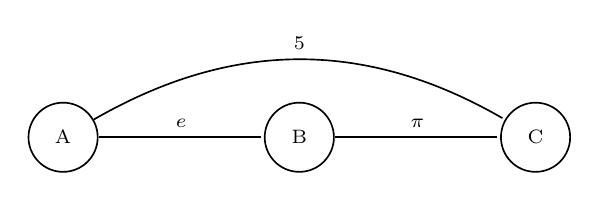
\begin{tikzpicture}[>=stealth',shorten >=1pt,auto,node distance=3cm,semithick]
	\tikzstyle{every state}=[draw=black,text=black]
	
	
	\node[state] (a)              {A};
	\node[state] (b) [right of=a] {B};
	\node[state] (c) [right of=b] {C};
	
	\path (a)   edge                  node {$e$} (b);
	\path (a)   edge [bend left]      node {$5$} (c);  
	\path (b)   edge                node {$\pi$} (c);

	\end{tikzpicture}}